%++++++++++++++++++++++++++++++++++++++++
\documentclass[letterpaper,12pt]{article}

\usepackage[margin=1in,letterpaper]{geometry}
\usepackage{amsmath}
\usepackage{graphicx}
\usepackage{booktabs}
\usepackage{cite}
\usepackage[final]{hyperref}

\hypersetup{
    colorlinks=true,
    linkcolor=blue,
    citecolor=blue,
    urlcolor=blue
}

\graphicspath{{results/}{results/v1_parameter_maps/}{../results/}{../results/v1_parameter_maps/}}
%++++++++++++++++++++++++++++++++++++++++

\begin{document}

\title{JWST Broad-Line AGN Growth Pilot at $z \geq 4$}
\author{Nicole Jiang}
\date{\today}
\maketitle

\begin{abstract}
\textit{Aims.} We construct a controlled v1 pilot catalogue of JWST broad-line accretion candidates at $z\geq4$ and use it to ask what simple seed-and-growth histories can reproduce the reported black-hole masses. The sample is intended as a reproducible test case, not a census of high-redshift accretion.

\textit{Methods.} We ingest a 34-row raw JADES broad-line AGN table from Juodzbalis et al. (2025), standardize source provenance and inference metadata, and retain 23 objects after applying the v1 $z\geq4$ filter. We evaluate each object with the implemented Dayal-style exponential growth model at fixed $z_{\rm seed}=30$, varying seed mass, average Eddington fraction, radiative efficiency, and a simple merger-boost factor.

\textit{Results.} The pilot sample spans $4.133 \leq z \leq 8.913$ and $6.06 \leq \log_{10}(M_{\rm BH}/M_\odot) \leq 8.57$. In the baseline $z_{\rm seed}=30$, $\epsilon=0.1$ case, fixed seed masses of $10^2$, $10^4$, and $10^5\,M_\odot$ require mean sample-average Eddington fractions of 0.718, 0.447, and 0.312, respectively. The most demanding object requires $f_{\rm Edd}=1.376$ for a $10^2\,M_\odot$ seed, but only 0.860 and 0.601 for $10^4$ and $10^5\,M_\odot$ seeds. Under a sub-Eddington $f_{\rm Edd}=0.3$, $\epsilon=0.1$ history, the median required seed mass is $\log_{10}(M_{\rm seed}/M_\odot)=4.78$.

\textit{Conclusions.} The v1 objects can often be accommodated by heavier seeds, lower radiative efficiency, or stronger average growth, but these diagnostics remain pilot-scale and should not be read as population-level evidence for any one seeding channel.

\textbf{Keywords:} high-redshift galaxies; black holes; active galactic nuclei; JWST; accretion; black-hole seeds
\end{abstract}

\section{Introduction}

JWST spectroscopy is now identifying accreting black-hole candidates during the first $\sim1.5$ Gyr of cosmic history. Such systems are useful because the time available for growth is short: an early massive black hole must have started from a sufficiently massive seed, accreted efficiently, formed early, grown through mergers, or combined several of these channels.

The challenge is that the relevant measurements are not always directly comparable across papers. Black-hole masses, host stellar masses, bolometric luminosities, and Eddington ratios can depend on line fitting, virial calibrations, bolometric corrections, and host--AGN decomposition. Because mass growth is exponential, even a modest systematic shift in $\log M_{\rm BH}$ can change the implied seed mass or average accretion requirement.

This paper therefore treats v1 as a deliberately narrow pilot. It standardizes one source class from one paper, JADES broad-line AGN from Juodzbalis et al. (2025), and uses the resulting catalogue to test a small set of transparent growth assumptions. The emphasis is reproducibility and interpretation hygiene before expanding to multiple source papers, duplicate-object handling, and broader candidate classes.

\section{Background Theory}

For fixed cosmology, the relevant clock is the difference between the cosmic age at observation and the cosmic age at seed formation. In the flat $\Lambda$CDM convention used here,

\begin{equation}
t(z) =
\frac{2}{3H_0\sqrt{\Omega_{\Lambda}}}
\operatorname{asinh}
\left[
\frac{\sqrt{\Omega_{\Lambda}/\Omega_m}}{(1+z)^{3/2}}
\right],
\label{eq:cosmic_time}
\end{equation}

with $H_0=70\,\mathrm{km\,s^{-1}\,Mpc^{-1}}$, $\Omega_m=0.3$, and $\Omega_\Lambda=0.7$. The growth interval is

\begin{equation}
\Delta t = t(z_{\rm obs}) - t(z_{\rm seed}),
\label{eq:delta_t}
\end{equation}

with $z_{\rm seed}>z_{\rm obs}$. This elapsed time is short at high redshift, so the same observed black-hole mass can imply different histories depending on the seed mass, average accretion fraction, radiative efficiency, and seed redshift. The calculations below use this dependence as a diagnostic tool rather than as a population model.

\section{Methods}

\subsection{Catalogue Construction}

The v1 catalogue is generated by ingesting \texttt{data/raw/v1\_raw.csv} and writing \texttt{data/processed/v1\_processed.csv} with \texttt{python -m scripts.process\_data}. The raw v1 table contains 34 rows. After the standard v1 redshift filter, $z\geq4$, the processed catalogue contains 23 rows.

All processed objects are JADES broad-line AGN from Juodzbalis et al. (2025), with source key \texttt{juodzbalis25\_jades\_blagn}. All 23 rows use \texttt{single-epoch-virial-halpha} black-hole masses. Nineteen of the 23 objects have BEAGLE host stellar masses, while all 23 have bolometric luminosities and reported Eddington ratios. Lensing magnification is absent for all processed objects and is explicitly tracked with the v1 missing-lensing flag. The quality flags divide the processed sample into 18 robust and 5 tentative entries.

The standardizer enforces the v1 schema before any growth calculation is performed. It validates required fields, numeric parsing, unique \texttt{measurement\_id} values, source provenance, optional missingness rules, and positive generated cosmic times. This keeps source-paper measurements and project-level interpretation separated.

\subsection{Growth Model}

The v1 notebook \texttt{scripts/v1\_evaluate.ipynb} evaluates the processed catalogue using \texttt{src/models.py} and \texttt{src/scoring.py}. The implemented growth equation is

\begin{equation}
M_{\rm BH}(t_{\rm obs}) =
M_{\rm seed}
\exp
\left[
f_{\rm Edd}
\frac{1-\epsilon}{\epsilon}
\frac{\Delta t}{t_{\rm Edd}}
\right],
\label{eq:bh_mass_growth}
\end{equation}

where $M_{\rm seed}$ is the initial seed mass, $f_{\rm Edd}$ is the time-averaged Eddington fraction, $\epsilon$ is the radiative efficiency, and $t_{\rm Edd}=c\sigma_T/(4\pi Gm_p)\simeq0.45\,\mathrm{Gyr}$ \cite{Dayal2024}. The elapsed time is $\Delta t=t(z_{\rm obs})-t(z_{\rm seed})$, computed with the flat $\Lambda$CDM convention in Equation~\ref{eq:cosmic_time} using $H_0=70\,\mathrm{km\,s^{-1}\,Mpc^{-1}}$, $\Omega_m=0.3$, and $\Omega_\Lambda=0.7$. V1 fixes $z_{\rm seed}=30$ for the diagnostic tables and figures.

Equivalently, the logarithmic mass gain is

\begin{equation}
\log_{10}\left(\frac{M_{\rm BH}}{M_{\rm seed}}\right)
=
\frac{1}{\ln 10}
f_{\rm Edd}
\frac{1-\epsilon}{\epsilon}
\frac{\Delta t}{t_{\rm Edd}}.
\label{eq:log_growth}
\end{equation}

The v1 scenario grid is intentionally compact. It compares each object to four seed ranges:

\begin{center}
\begin{tabular}{ll}
\toprule
Label & Seed-mass range \\
\midrule
Light / Pop III-like & $10^1$--$10^2\,M_\odot$ \\
Intermediate / cluster-like & $10^3$--$10^4\,M_\odot$ \\
Heavy / DCBH-like & $10^4$--$10^6\,M_\odot$ \\
PBH-like diagnostic range & $10^2$--$10^6\,M_\odot$ \\
\bottomrule
\end{tabular}
\end{center}

These labels are used as interpretive bins, not as population priors. The same grid is evaluated for four interpretation variants: the baseline catalogue values, $\log_{10}M_{\rm BH}$ shifted by $-0.3$ dex, $\log_{10}M_{\rm BH}$ shifted by $+0.3$ dex, and a 20 percent AGN-contamination correction to the host stellar mass where $M_\star$ is available. The host-mass correction changes the black-hole-to-stellar-mass ratio but does not alter the black-hole growth calculation.

The growth configurations are $f_{\rm Edd}=1$ with $\epsilon=0.1$, $f_{\rm Edd}=0.3$ with $\epsilon=0.1$, $f_{\rm Edd}=2$ with $\epsilon=0.05$, and $f_{\rm Edd}=1$ with $\epsilon=0.1$ plus a merger boost $B_{\rm merge}=2$. In addition to these fixed-growth calculations, v1 solves for the required average $f_{\rm Edd}$ at fixed seed masses of $10^2$, $10^4$, and $10^5\,M_\odot$.

\section{Results}

\subsection{Catalogue Properties}

The processed v1 sample contains $N=23$ objects. It is a homogeneous JADES broad-line AGN pilot sample, not a high-redshift accretion census. The redshifts span $4.133 \leq z \leq 8.913$, with median $z=5.480$. In the adopted flat $\Lambda$CDM convention, the cosmic age at observation spans 0.545--1.458 Gyr.

The standardized black-hole masses span $6.06 \leq \log_{10}(M_{\rm BH}/M_\odot) \leq 8.57$, with median $\log_{10}(M_{\rm BH}/M_\odot)=7.33$. Reported Eddington ratios span 0.015--0.38, with median 0.11. Host stellar masses are available for 19 objects and span $7.40 \leq \log_{10}(M_\star/M_\odot) \leq 10.93$. For those 19 objects, the black-hole-to-stellar-mass ratio has median $\log_{10}(M_{\rm BH}/M_\star)=-1.73$ and range $-3.23$ to $-0.07$.

These reported Eddington ratios describe source-paper measurements, while the growth-model diagnostics ask a different question: what average accretion history could have built the inferred black-hole mass from an assumed seed?

\begin{figure}
    \centering
    
\includegraphics[width=0.95\linewidth]{v1_mbh_vs_redshift_growth_tracks.png}
    \caption{V1 black-hole masses compared with constant-accretion growth tracks. Points are catalogue black-hole masses with reported mass uncertainties. Curves start at $z_{\rm seed}=30$; colour marks seed mass and line style marks constant average $f_{\rm Edd}$. Objects above a track require a heavier seed, higher average accretion, lower radiative efficiency, earlier seeding, or additional growth channels.}
    \label{fig:growth_tracks}
\end{figure}

\subsection{Fixed-Seed Requirements}

For the baseline $\epsilon=0.1$ case without a merger boost, the mean required average $f_{\rm Edd}$ is 0.718 for $10^2\,M_\odot$ seeds, 0.447 for $10^4\,M_\odot$ seeds, and 0.312 for $10^5\,M_\odot$ seeds. The corresponding maximum object-by-object requirements are 1.376, 0.860, and 0.601. Lowering the efficiency to $\epsilon=0.05$ reduces these mean requirements to 0.340, 0.212, and 0.148 for the same seed masses. Adding a factor-of-two merger boost gives mean requirements of 0.677, 0.407, and 0.271.

Thus, within this pilot sample, light $10^2\,M_\odot$ seeds are sometimes pushed into mildly super-Eddington average-growth territory under the baseline setup, while $10^4$--$10^5\,M_\odot$ seeds remain below $f_{\rm Edd}=1$ for all v1 objects in the same calculation.

\subsection{Fixed-Growth Requirements}

Solving instead for the required seed mass gives a complementary view. With $f_{\rm Edd}=0.3$ and $\epsilon=0.1$, the median required seed mass is $\log_{10}(M_{\rm seed}/M_\odot)=4.78$, with an object-by-object range from 2.80 to 6.75. This places the median requirement in the heavy-seed scale, while the upper end extends above $10^6\,M_\odot$.

For $f_{\rm Edd}=1$ and $\epsilon=0.1$, the formal median required seed mass is below one solar mass. This is not a physical seed-mass inference; it indicates that the assumed growth history is more than sufficient for many objects and would need to be moderated by lower average accretion, later seeding, higher radiative efficiency, or other changes. The $f_{\rm Edd}=2$, $\epsilon=0.05$ case is even more overproductive in this formal sense.

\begin{figure}
    \centering
    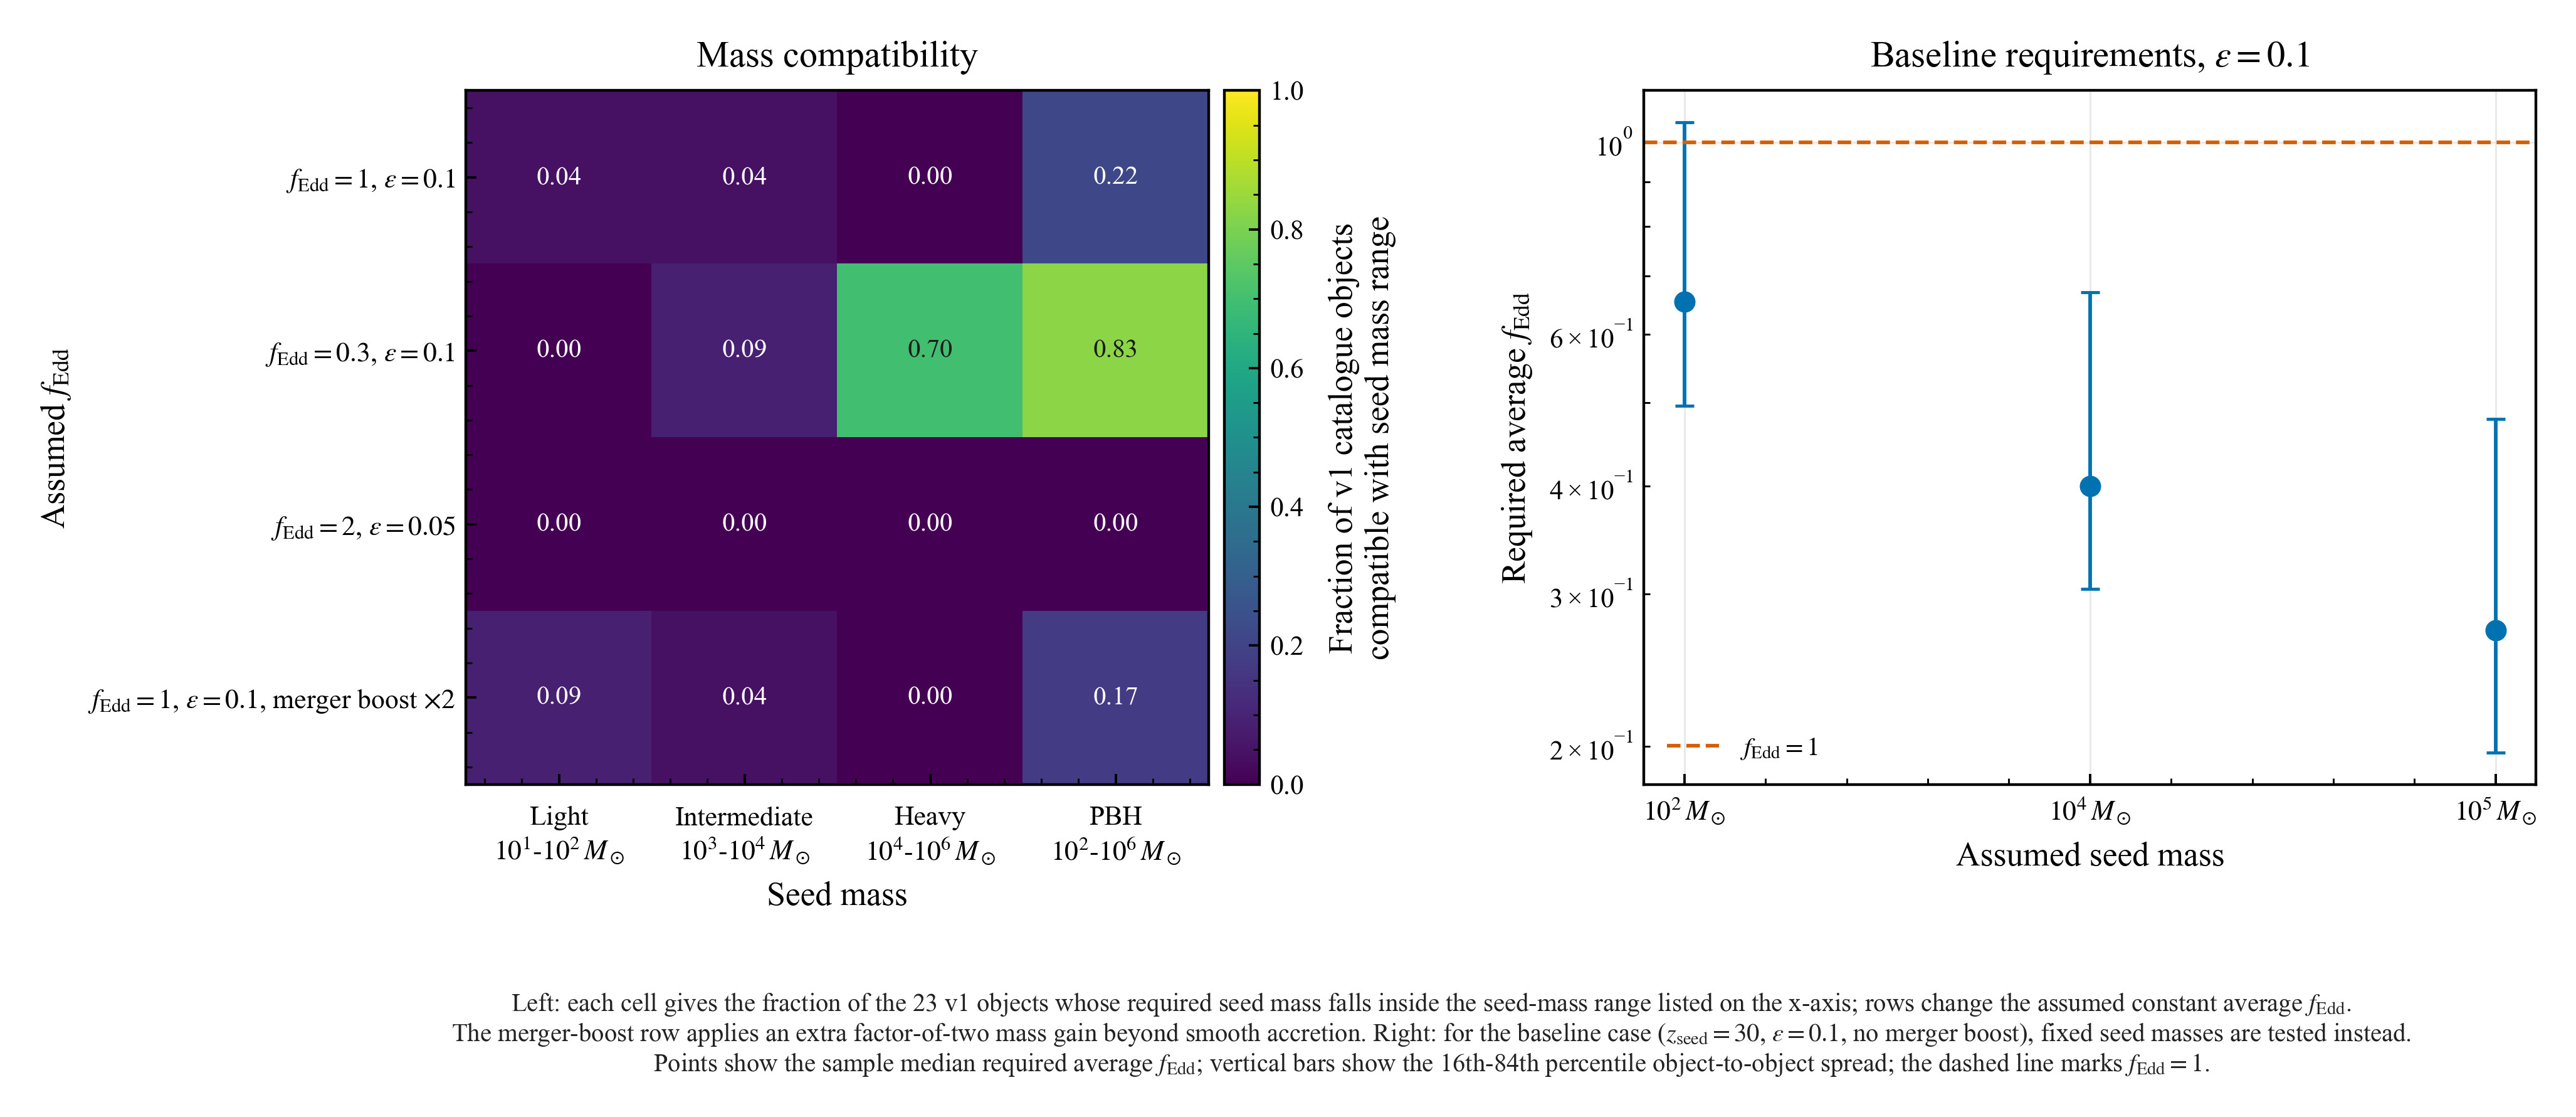
\includegraphics[width=0.98\linewidth]{v1_sample_compatibility_summary.png}
    \caption{Sample-level compatibility diagnostics. Left: fraction of the 23 v1 objects whose required seed mass falls inside each seed-model range for the listed growth assumptions. Right: baseline required average $f_{\rm Edd}$ for fixed seed masses, with points showing sample medians and vertical bars showing object-to-object spread. The heatmap is a diagnostic summary rather than a probability model.}
    \label{fig:compatibility_summary}
\end{figure}

\subsection{Parameter Maps}

The notebook also generates one parameter-space map per object. Each map shows predicted $\log_{10}(M_{\rm BH}/M_\odot)$ in the plane of $\log_{10}(M_{\rm seed}/M_\odot)$ and average $f_{\rm Edd}$ for fixed $z_{\rm seed}=30$ and $\epsilon=0.1$, with contours marking the observed mass and reported mass uncertainty.

\begin{figure}
    \centering
    
\includegraphics[width=0.75\linewidth]{v1_parameter_map_gn38509-juodzbalis25.png}
    \caption{Example per-object parameter map for GN-38509, the most massive object in the v1 catalogue. The solid contour marks the reported black-hole mass, dashed contours mark the reported mass uncertainty, and dotted vertical lines mark seed-mass reference scales.}
    \label{fig:parameter_map_example}
\end{figure}

These maps are useful because they show the continuous degeneracy behind the table summaries. For a fixed observed mass, moving to heavier seeds lowers the required average $f_{\rm Edd}$, while moving to lighter seeds raises it. The current v1 maps should be read as controlled single-object diagnostics, not as evidence that the sample is complete or representative.

\section{Discussion}

The v1 exercise demonstrates the value of keeping data standardization and growth interpretation separate. The standardized catalogue records what was reported and how it was inferred; the model layer then asks how those reported values behave under shared assumptions. This avoids mixing source-paper measurements with project-level interpretation.

The pilot results also show why the word ``candidate'' matters. The source sample is a broad-line AGN subset from one survey programme and one paper. It is not a uniform census of all high-redshift black holes, nor does it include the duplicate handling, multi-paper measurement comparison, or uncertainty propagation planned for later versions. The feasibility scores and heatmaps are therefore best used to identify which objects and assumptions deserve closer inspection.

Within these limits, the v1 outputs are internally consistent with a simple picture: light seeds require stronger sustained average growth, while intermediate and heavy seeds reduce that burden. Some high-redshift or high-mass objects remain the most informative stress tests because their available growth time is short or their inferred black-hole mass is large.

\section{Conclusions}

This work turns the current repository into a concise v1 manuscript built around three reproducible products: a standardized source-tracked catalogue, analytic seed-and-growth calculations, and diagnostic figures. The main conclusions are:

\begin{enumerate}
    \item The v1 catalogue contains 23 JADES broad-line AGN at $4.133 \leq z \leq 8.913$, with 18 robust and 5 tentative rows.
    \item Baseline fixed-seed calculations show that $10^4$--$10^5\,M_\odot$ seeds can reproduce all v1 objects with average $f_{\rm Edd}<1$ for $z_{\rm seed}=30$ and $\epsilon=0.1$, while $10^2\,M_\odot$ seeds require mildly super-Eddington average growth for the most demanding cases.
    \item Under $f_{\rm Edd}=0.3$ and $\epsilon=0.1$, the median required seed mass is $\log_{10}(M_{\rm seed}/M_\odot)=4.78$, placing the typical requirement in the heavy-seed scale.
    \item These results should be treated as a controlled pilot analysis, not as population-level evidence for or against a seeding channel.
\end{enumerate}

\begin{thebibliography}{99}

\bibitem{Dayal2024}
Dayal, P. 2024,
\textit{Astronomy \& Astrophysics}, 690, A182.
\href{https://www.aanda.org/articles/aa/full_html/2024/10/aa51481-24/aa51481-24.html}{A\&A article}

\bibitem{Juodzbalis2025}
Juodzbalis, X., et al. 2025,
\textit{JADES: comprehensive census of broad-line AGN from Reionization to Cosmic Noon revealed by JWST},
MNRAS, arXiv:2504.03551.
\href{https://arxiv.org/abs/2504.03551}{arXiv article}

\end{thebibliography}

\appendix

\section{Derivation of the Cosmic Time Relation}

Start from flat $\Lambda$CDM:
\[
t(z)=\frac{1}{H_0}\int_z^\infty
\frac{dz'}{(1+z')\sqrt{\Omega_m(1+z')^3+\Omega_\Lambda}}.
\]

Let
\[
a\equiv \frac{1}{1+z},\qquad a'\equiv \frac{1}{1+z'},\qquad
dz'=-\frac{da'}{a'^2}.
\]

Then
\[
t(a)=\frac{1}{H_0}\int_0^a
\frac{da'}{a'\sqrt{\Omega_m/a'^3+\Omega_\Lambda}}
=
\frac{1}{H_0}\int_0^a
\frac{\sqrt{a'}\,da'}{\sqrt{\Omega_m+\Omega_\Lambda a'^3}}.
\]

Let
\[
u\equiv \sqrt{\frac{\Omega_\Lambda}{\Omega_m}}\,a'^{3/2},
\]
so that
\[
du=\sqrt{\frac{\Omega_\Lambda}{\Omega_m}}\frac{3}{2}a'^{1/2}da',
\]
and therefore
\[
a'^{1/2}da'=\frac{2}{3}\sqrt{\frac{\Omega_m}{\Omega_\Lambda}}\,du.
\]

Since
\[
\sqrt{\Omega_m+\Omega_\Lambda a'^3}
=
\sqrt{\Omega_m}\sqrt{1+u^2},
\]
we obtain
\[
t(a)=
\frac{1}{H_0}
\frac{2}{3\sqrt{\Omega_\Lambda}}
\int_0^{u(a)}
\frac{du}{\sqrt{1+u^2}}.
\]

Thus
\[
t(a)=
\frac{2}{3H_0\sqrt{\Omega_\Lambda}}
\operatorname{asinh}\!\big(u(a)\big),
\]
where
\[
u(a)=
\sqrt{\frac{\Omega_\Lambda}{\Omega_m}}\,a^{3/2}.
\]

Using $a=(1+z)^{-1}$ gives
\[
\boxed{
t(z)=
\frac{2}{3H_0\sqrt{\Omega_\Lambda}}
\operatorname{asinh}
\left[
\frac{\sqrt{\Omega_\Lambda/\Omega_m}}{(1+z)^{3/2}}
\right]
}.
\]

\section{V1 Repository Outputs}

The manuscript numbers are taken from the repository outputs available at draft time:
\texttt{data/processed/v1\_processed.csv},
\texttt{results/v1\_evaluation\_table.csv},
\texttt{results/v1\_required\_fedd\_by\_seed\_mass.csv},
\texttt{results/v1\_required\_mseed\_by\_growth\_assumption.csv},
\texttt{results/v1\_sample\_summary.csv},
\texttt{results/v1\_mbh\_vs\_redshift\_growth\_tracks.png},
\texttt{results/v1\_sample\_compatibility\_summary.png}, and the 23 per-object PNG files in \texttt{results/v1\_parameter\_maps/}.

\end{document}
